\documentclass{article}
\usepackage[utf8]{inputenc}
\usepackage{amsmath}
\usepackage{graphicx}
\usepackage{xcolor}
\usepackage{hyperref}
\usepackage{natbib}
\bibliographystyle{plainnat}
\title{Our Spatial Paper}
\author{Your Name}
\date{\today}

\begin{document}

\maketitle

\begin{abstract}
    Please be concise.
\end{abstract}

\section{Project Plan}
\begin{itemize}
    \item Idea Formation and Lit Review  Jan 13-17  [together ]
    \item Theory - Coming up with a Model/Try to meet with Esteban to get feedback? Jan 20-22 [together]
    \item Theory - Solving the Model Jan 23-24 [Key Person = Henrique]
    \item Coding (data, estimation, counterfactual, and results) - Jan 27 - Jan 31  [Key Person = ]
    \begin{itemize}
        \item Inputs are fairly divisible
        \item Outputs are less divisible
        \item Writing -  Feb 4 - 7  (KeyPerson)
   \end{itemize}
\end{itemize}
\section{Meeting Notes}
\begin{enumerate}
    \item  Could have teams of (2) for various things. 
    \item There are some tasks that are independent. 
    \item Decide to break stuff up once we actually have an idea.
    \item Henrique: Likes Lit Review / Idea Formation / Likes Writing [let us simplify model if possible]. Prefers the equilibrium part of coding to the early / data cleaning part Less good at Geodata.  Very good at polishing and visual details. 
    \item Jeffrey: Likes Coding / Likes Writing
    \item Yulia: Interested in counterfactuals part of coding. Curious about theory. Experience about writing / likes writing. 
\end{enumerate}

\subsection{ for next meeting, Jan 17 }
\begin{enumerate}
    \item Read model / counterfactuals of Monte et al in detail enough 
    \item In the Esteban choose your model 
    \item Map Monte et al to Esteban's choose your model. 
    \item Look at Jeffrey's ideas. 
\end{enumerate}



\subsection{During next meeting}
\begin{enumerate}
    \item pick idea
    \item assign data 
\end{enumerate}


\section{Introduction}
\label{sec:intro}
Your introduction here.

\section{Background and Diagnostic}
Prompt:Why is the question or policy you want to examine
important? Why is a quantitative spatial model the right tool to answer the question?
Are there any particular features of the policy/economic environment that are impor-
tant for the analysis? Feel free to focus on one or a few aspects that you want to study
in depth and identify the underlying mechanisms, which will inform you about the key
elements to be included in your model.
\subsection{Brainstorming }

\subsubsection{Idea 1: Self-driving cars}
The original invention of the internal combustion engine
radically transformed rents, population density, and the distribution of economic activity. 

The rise of self-driving cars is likely to have a similar transformative effect on the spatial distribution of economic activity.
Waymo currently operates self-driving cars in Phoenix, Arizona, Los Angeles, CA, and San Francisco, CA.



Our first counterfactual will thus be the introduction of self-driving cars in these three counties, which collectively comprise 
XYZ share of the US population, and  \$PQR share of GDP.

Our second counterfactual will be to introduce self-driving in all counties.

Our third counterfactual, which is most policy-relevant, will be the introduction of self-driving in the top [XXX\%] of counties by some measure of regulatory friendliness.
 This will allow us to study a setting where a sizable chunk of the US economy has self-driving, and the rest doesn't. This is inspired by the real-world heterogeneity in regulations, compare, e.g. California and Arizona to, e.g., New York.
 
 his will let us speak to distributional effects (welfare, rents, population) of heterogeneity in self-driving car regulation.

\textcolor{red}{Fundamentally, this amounts to what do you mean by ``introduction''? 100\% use of car trips become this?
does any walking or biking or public transit substitute towards this?}

With American Time Use Data, which not only reports how much time people spend on various activities, but how much they like or dislike them, we can microfound the cost of commuting (maybe there is another paper we can take this from, instead, too), and building on YYY paper, which compares the cost of commuting by public transit vs. cars, 
we can back out how the primitives of commuting costs change in XYZ locations.



Important things here:
\begin{enumerate}
    \item Isn't it obvious that a decline in commuting costs would lead people to spread out? Does it matter that it's self-driving cars causing this decline? 

    \item Do you model the choice of how to commute, or just reduced-form things?
\item Just reducing $\kappa_{ni}$ for these places seems a little lazy
\item Might the interesting angle to be quantify how places that are slow-to-allow self driving cars ``fall behind'', in some sense, those which are faster to allow it? 
\item Do we think that (me using a self driving car) has a positive externality on other people?
\item Any pecuniary costs in the counterfactual (e.g. I have to buy a self driving car), or just the commuting costs?
\item Will self-driving have a homogeneous effect on all $\kappa_{ni}$? Probably should only apply to certain node-pairs where people are driving.
\end{enumerate}


\subsubsection{Data and Feasibility for SelfDriving}
Goal here is to justify how much to reduce $\kappa_{ni}$ in places where self-driving cars are reduced.

Remember.

$$\kappa_{ni} \propto dist_{ni}^{-\phi}$$

We would have to choose a different parameterization. 

The simplest possible change would be to just assume everyone commutes by driving, and include a ``switching parameter'' for self-driving:


Assuming 100\% of people commute by car
$$\kappa^{SelfDrive}_{ni} \propto ( (U_{commute}/U_{TV} )  dist_{ni} ) ^{-\phi}$$

$$\kappa^{NoSelfDrive}_{ni} \propto ( dist_{ni} ) ^{-\phi}$$

where we get $U_{self drive}$ and $U_{ TV}$ from the Day Reconstruction Method . People rates

Watching TV with 4.19 positive affect, 0.58 negative affect. Commuting as 3.45 positive affect, 0.89 negative affect.

$$\frac{3.45 - 0.89}{ 4.19-0.58} = 71\%$$
(A lot of assumptions may neeed to assume a cardinal interpretation of these ordinal rankings...)
So commuting costs are lowered to  $\approx 71\%$ of their former value.

A more sophisticated analysis would:

\begin{enumerate}
\item Separate psychological and monetary costs of commuting (depreciation on car, gas.) - probably not too important since monetary costs wouldn't be changing in the counterfactual. Overall, not including this OVERESTIMATES the decline in commute costs. 
\item Recognize Yulia's point that people also probably *get there faster* (not just get there while watching TV). Not including this UNDERESTIMATES the decline in commute costs. 
\item Not assume 100\% of people drive, and instead base this on data on commute modes, given by the ACS table (see Github data folder). Assuming 100\% OVERSTIMATES the decline in commute costs. However, to get pretty close to this we could use the population-weighted average, which seems to be about 77\%. \href{https://www2.census.gov/library/publications/2024/demo/acsbr-018.pdf}{source}. Denote this $s_{driving}$
\end{enumerate}

Doing the last one seems feasible and would just modify our calc to be as follows:

Assuming $s_{driving}$ \% of people commute by car
$$\kappa^{SelfDrive}_{ni} \propto ( [s_{driving}\frac{U_{commute}}{U_{TV}}  + (1-s_{driving}) (1) ] dist_{ni} ) ^{-\phi}$$

So, of course, if $s_{driving}=0$ we don't modify that county-pair's commute costs at all. 


Counterfactual:
 ``Adoption'' here just means what percent of the way we reduce their commute costs to the self-driving level. (see above)
 Since regulation is at the state-level we need to take care.
 %Or we could reduce it based on the average level of regulation in the two-state pairs.
 In reality, it probably will be the more regulated state for any county-pair, which matter.
 So probably we should just use the max. regulation of every county pair to determine how much to reduce commute costs. 
\begin{enumerate}
    \item Luckily, the way counties work is they're only in one state (impossible to have a county cross state borders)
\item Easiest is to assume Self-Driving is fully adopted in Arizona, California, Texas, and Florida (all county-pairs fully adopt in those states i.e. use $\kappa^{self-drive}$, every other county pair is not modified)
\item More interesting would be a gradient of adoption. We could impose that the most friendly state fully adopts (100\%), as above, and least friendly doesn't adopt at all (0\%). . I got a 50 state list from ChatGPT (see figures) which we could use for starters, in the data folder. It accords with intuition: CA, TX, FL, NV, AZ all either highest or second-highest rating.

\end{enumerate}

\begin{figure}
        \centering
        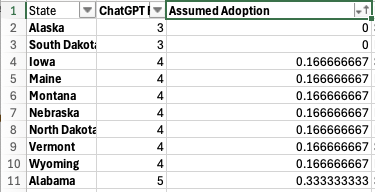
\includegraphics[width=0.5\textwidth]{img/strict.png}
        \caption{Strictest / lowest adoption}
\end{figure}

\begin{figure}
    \centering
    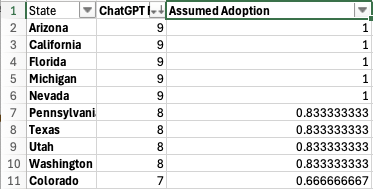
\includegraphics[width=0.5\textwidth]{img/friendly.png}
    \caption{Friendliest / highest adoption}
\end{figure}



\subsubsection{Idea 2: Incorporating car ownership}
Who owns cars, where, and why?

Is the cost of car ownership incorporated into the indifference conditions of these spatial models: maybe chicago isn't actually much cheaper than e.g. nyc once you add a car payment to your rent [which many more people seem to have / beed in Chicago] 


Kind of tricky. Need some heterogeneity to endogenize this choice which already complicates things.

Could have $\kappa^{car}_{ni}$ <
$\kappa^{no \ car}_{ni} $ and people choose to pay a fixed cost for a car or not. 
Then, who gets a car vs. who doesn't? 
People who have higher preference for space, $\alpha_i$

Could just have a owning a car as an effective decline in wage (rather than an asset).
If we wanted to really get fancy, we could have heterogeneous commuting costs, i.e. weight or power $\kappa_{ni}$ by something. 


\subsubsection{Idea 3: }
I wonder if Amazon has impacted car ownership through making it easier to just have a bunch of stuff delivered. 
And this in turn reduces congestion? Seems second-order, maybe not.

\subsubsection{Idea 4: Crime $\rightarrow$ Commuting}
My intuition is that, all else equal, people take public transit less in a city if crime ( LA buses, for example, Chicago red line, more recently, NY Subway).

Does this impose a quantitatively important externality on commuting costs, by shifting people to cars?

In a complete paper, we would endogenize crime, by also examining how available commuting influences crime, as well. 

\subsubsection{Idea 5: Weather, Commuting Costs, and Climate Change}
Climate change may have 

distributional consequences on commuting costs:
places like Florida may see more precipitation. Places like Chicago may see fewer snowy days [citation needed]
\subsubsection{Idea 6: Zoning in car cities vs walkable cities}

\subsubsection{Idea 7: Distributional Efects of parking requirements}
Maybe minimum parking requirements in business areas let fewer people live in the city, but lowers commute times for the people that do commute.
\subsubsection{Idea 8: Car safety and commuting}
\begin{figure}
    \centering
    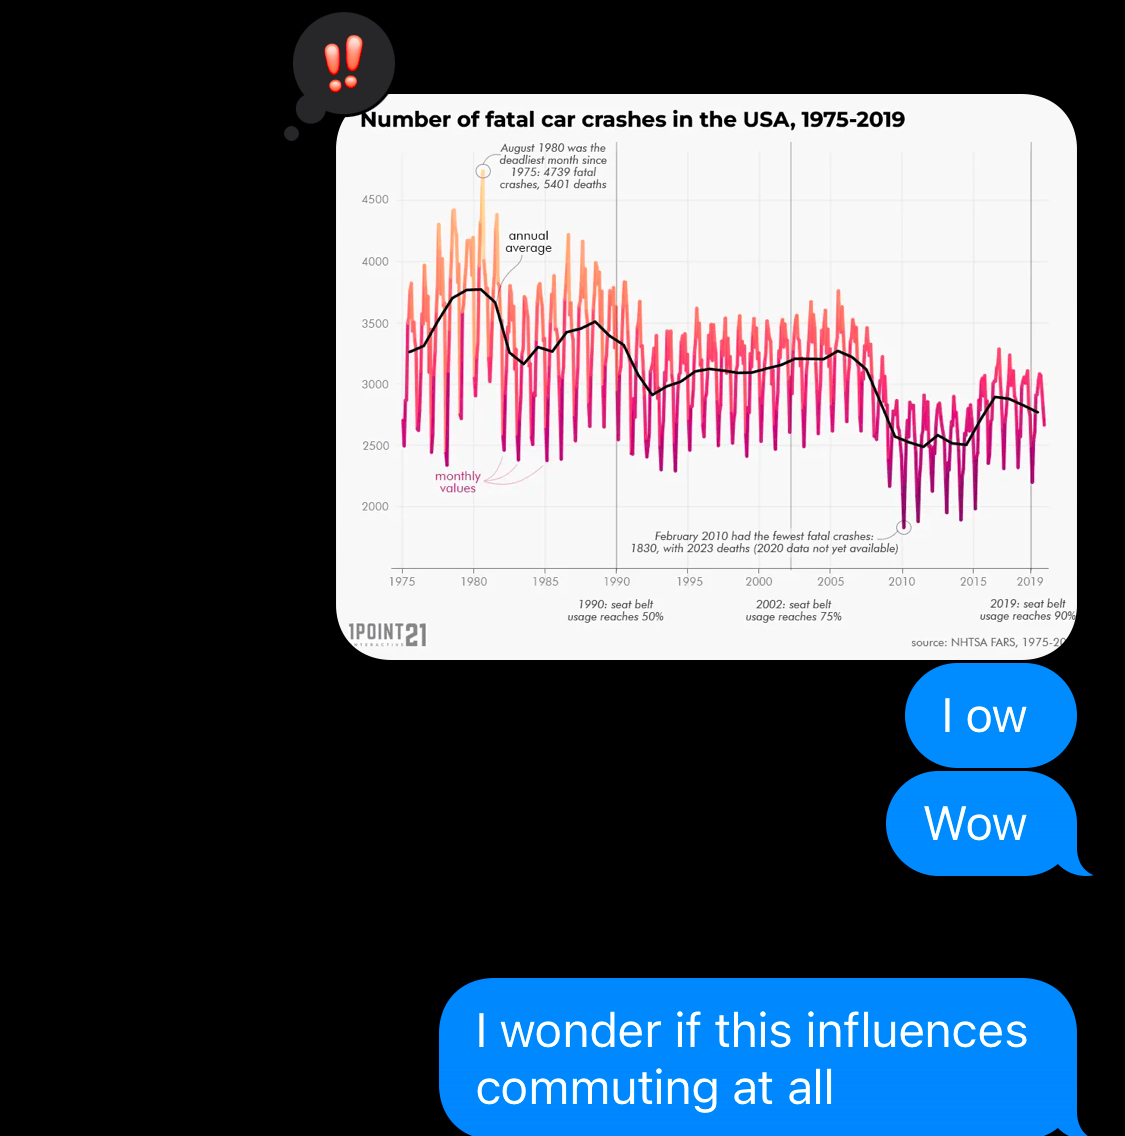
\includegraphics[width=0.5\textwidth]{img/cardeaths.jpeg}
    \caption{Deaths per capita in the US from car accidents.}
    \label{fig:car_deaths}
\end{figure}


\subsubsection{Yulia's Ideas}
nat.  disasters, housing voichers
\begin{enumerate}
\item money costs
\item time costs
\item enjoyment of time ? 
\end{enumerate}
\subsubsection{Henrique}
\begin{enumerate}
\item Simple addition of trains etc.
\item Work from home? 
\end{enumerate}

\section{Model}

\subsection{Jeff's notes on Monte et al model}
\begin{enumerate}
\item It's a bit weird to have this `E[]' component. WTF. Are we treating it as random which place they commute to? Yes.
\item Amenities are our idiosyncratic term and are paramterized by $b_{ni\omega}$, that they can differ by person and where they live / work. Or better, put: they each get $N^2$ shocks.
\item Goods - standard
\item Closing the land market: landlords own everything.
\item People's utility is just in land. So there's no housing being created people just eat $C$ and $H$.
\item  When can we use exact hat algebra for counterfactuals? (see Eqn. 24)
\end{enumerate}

Write down the model that directly speaks to the mechanisms you identified
in the previous step. You need to specify all the building blocks and solve for the
equilibrium (equilibria). Please be clear and concise, and feel free to leave tedious
derivations in the appendix or cite any relevant derivations you want to lift from
existing papers.
You are encouraged to tweak or simplify an existing model, like the one in Monte et
al. (2018). If you want to be more creative, feel free to select components from the
“menu of quantitative spatial models” in Section 2 of Redding and Rossi-Hansberg
(2017). When tweaking an existing model or building a model of your own, make
sure you include only the necessary elements related to your proposed mechanisms.
Importantly, please be aware of the time and feasibility constraints when specifying
your model.
\subsection{Mapping Monte et al to Redding Rossi Hansberg 2017}
\begin{enumerate}
\item 2.1 - Preferences: Love of Variety (CES), Single Sector, Exogenous Amenities, Fixed Land (enters into utility), Idiosyncratic Preferences
\item 2.2 - Increasing Returns (kinda. TFP is constant, but there's a fixed cost), Exogenous productivity differences, No input-output linkages, No fixed factors in production (only labor)
\item 2.3 - Variable trade costs (ice berg), asymmetry allowed, economic and geographic frictions (i.e. no stand on what's causing trade costs). Only land is not traded.
\item 2.4 - No knowledge externalities. Exogenous local productivity. No transferability of ideas. 
\item 2.5 - No migration costs , Yes commuting costs, No heterogeneity (beyond idiosyncratic preferences), No congestion
\item 2.6 - Homogeneous labor (no skill endowments), Exogenous land, in Counties in the US, No capital
\item 2.7 - Market Structure = Monopolistic Competition, General Eqm, Land ownership: Owned by immobile landlords who spend income locally (no need to ``track'' workers, but also no externality from moving on other people) , Trade Balance: Deficits/Surplus permitted but only exist due to commuting? \footnote{Kind of vague on this still? Monte et al explanation ``a location’s total workplace income equals total expenditure on the goods that it produces, total residential income can differ from total workplace income (because of commuting).''} , 
\item 
\end{enumerate}

\subsubsection{Simplifications to Monte et al}
\begin{enumerate}
\item do we need monopolistic competition or would CRS be easier? 
\item honestly hard to get a much simpler model than this if you want trade in goods and commuting. Good job Esteban.
\end{enumerate}

\subsubsection{Monte et al and the Data}
We might be able to not know some of these with Exact-Hat magic. I will try to note that if so.
I am also sometimes being a little vague when I'm talking about model vs. data, sorry.

Structural parameters
\begin{enumerate}
\item $\alpha$, Cobb Douglas weight on consumption goods, 60\%, taken from the BEA (rest is housing)
\item $\epsilon$ dispersion of amenities (estimate later, at 3.3)
\item $\sigma$ CES Elasticity of Substitution = 4 (central value in literature)
\item $F$ fixed cost of production (maybe? we never seem to actually need this so I guess it gets exact-hatted out or cancels with itself or something)
\end{enumerate}
Calibrated parameters
\begin{enumerate}
\item Wages $w_i$ (totally exogenous in this model, not even calibrated, I think - we just take the county mean from the data and that's our wage vector)
\item $d_{ni}$ goods trade cost (compute this as a detrministic function of distance a la Allen Arkolakis 2014)
\item $\kappa_{ni}$, commuting costs
\item $A_i$ productivity vector
\item $B_{ni}$ exogenous amenities from living in $n$ and working in $i$ (why have this be a matrix? can we simplify this? maybe we're underidentified if so)
\end{enumerate} 

Equilibrium objects
%Quantities Taken from the Data /  Estimating Equations ?...

Note in this model, $i$ is where you work, $n$ is where you live.
\begin{enumerate}
\item $H_n$ housing stock
\item $L_i$ labor force
\item $R_n$ residents [note, having an $R$ distinct from $L$ is what makes this a commuting model!]
\end{enumerate}

The below can be expressed using all of the above (I would call them ``derived equilibrium objects'')
\begin{enumerate}
\item $M_i = L_i/(\sigma F)$ varieties produced
\item $P_n$ price index
\item $Q_n$ price of land
\item $\lambda_{ni}$ probability of working in $i$ and living in $n$ (unconditional probability), there are some nice eqm objects
\item $\pi_{ni}$ share of location $n$ expenditure on goods produced in $i$
\item $\bar v_n$ average residential income (differs from wages due to commuting)
\end{enumerate}

\subsubsection{Taking the model to the data}


\begin{enumerate}
    \item We basically have data on $R_n$, $L_i$, $\bar v_n$, 
    \item While we don't have $\pi_{ni}$ , we have a 123x123 matrix of CFS regions, and we allocate the deficit for each CFS region across the countries within that region according to their shares of the CFS region's income
\item  We are going to calibrate $A_i$, $d_{ni}$, $\kappa_{ni}$ to match wages, commuting flows, and populations.
\end{enumerate}

Parameterizing $d_{ni}$ (I say parameterizing because there is no economics here, just geography and math)
This is more in the line of Allen Arkolakis 2014 where you calculate trade costs than the Regional Sector Model where you back out trade costs.

\begin{enumerate}
\item $(d_{ni})^{1-\sigma} = dist_{ni}^{-\psi (1-\sigma)} $ (the $\tilde e$ thing turns out not to matter I think)
\item Since we take $\sigma$ from the lit. all we need to do is calc $\psi$ and get some data on distances.
\item we can do that using a gravity regression - of trade flows onto destination and origin fixed effects, and distance. The parameter on distance is going to be 
$-(\sigma-1)\psi$
\item They get $-1.29 = -(\sigma-1)\psi$ so $\psi = 0.43$. Probably good to make sure we get this same thing with their data !! \textcolor{red}{Validation Check}
\item Okay, so we have $d_{ni}$
\end{enumerate}
\textcolor{red}{It's a bit buried, but I believe this means symmetric trade costs! (as long as their distance measure is symmetric)}

Solving for $A_i$
\begin{enumerate}
\item Can get a system of $N$ equations N unknowns ,eq (16) in the paper,  (wages, employment, residents, avg residential income and trade deficits are or computed fairly immediately from data)
\item Computationally, we would like to do a contraction mapping thing right? But I don't know that it is a contraction..They give the excess demand equation in the appendix. 
\end{enumerate}

Onto commuting stuff... we can solve for $\lambda_{ni}$ as $N^2$ system of equation with same number of unknowns.


The thing we are gonna be solving for is $\mathcal{B}_{ni} = B_{ni}\kappa_{ni}^{-\epsilon}$ (I am guessing we cannot identify $\kappa$ (distance) and $B$ (amenities) separately)



First we need to estimate more parameters though!

We are going to parameterize $\kappa_{ni}$ as a function of distance $(dist)^{-\phi}$, like we did with goods costs before but with another parameter $\phi$ instead of $\psi(\sigma-1)$. This will let us recover $\epsilon$ in a 2-step process. 

\begin{enumerate}
\item Estimate $\phi$ with a gravity regression (they get $\phi = 4.43$) (B.74 in appendix)
 \item Then I guess using $\phi$ and some features of their model compute $\epsilon=3.3$ in another regression (B.75 in appendix)
\end{enumerate}

Then you use $R_n$, $H_n$, $v_n$, $w_n$,  $\pi_{nn}$ (don't need the whole matrix!), $L_n$
to solve for $\lambda_{ni}$.
\subsubsection{How do counterfactuals work / Exact-Hat Notation }


(from shock to commuting costs,they say what they assume is held fixed that permits this eqn to work)
\begin{equation}
\hat{U} = \left(\frac{1}{\tilde{\lambda}_{ii}}\right)^{\frac{1}{\epsilon}} \left(\frac{1}{\tilde{\pi}_{ii}}\right)^{\frac{\alpha}{\sigma-1}} \left(\frac{\hat{w}_i}{\hat{v}_i}\right)^{1-\alpha} \frac{\hat{L}_i^{\frac{\alpha}{\sigma-1}}}{\hat{R}_i^{1-\alpha}}
\end{equation}

\section{Data and Estimation}
\label{sec:data}
Describe the data you use to estimate the model. What
variables do you need? How do you access them? How do you plan to estimate the
model? For parameters that you will calibrate, justify your choices. For parameters
that you will estimate, explain your strategy.

\subsection{Notes on what Monte et al do - -Jeffrey}
This paper mostly uses 2007 data. We could probably update it, or could not if we want to be able to compare numbers for sanity.
Section D of the Appendix is amazing.
Commodity Flow Survey (CFS)

- Bilateral trade between 123 CFS regions (123 x 123) $\implies$ 123-long vector of trade deficits, which are then allocated to the 3,111 counties in a particular way (pro rata share of residential income). (why, only need to allocate deficits, rest stays there? )

- Bilateral distance shipped - ?? used for why? I think it's just some random Appendix analysis. [As a check on this specification, we aggregate the model’s predictions for trade between counties within pairs of CFS regions, and compare these predictions to the data on CFS bilateral trade] (why can't we just use county centroids)... they don't need to for calibrating $\psi$ .. % might only be used in calibrating $\psi$.. or might not be used at all. ``We use the model’s gravity equation and observed bilateral trade between CFS regions to estimate the composite parameter $-\psi(\sigma-1)$'' .. or might just be used as a check (As a check on this specification, we aggregate the model’s predictions for trade between counties within pairs of CFS regions, and compare these predictions to the data on CFS bilateral trad)

American Community Survey (ACS)

- Commuting probabilities between counties (3111 x 3111) .. 
Bureau of Economic Analysis

- Employment by workplace county (3111 vector) $\implies$ (multiplying / dividing by commuting probabilities, and Residents of each county) [This is important! We do not directly use data on number of residents of each county , just number of workers. This ensures internal consistency of Num Residents and Num Workers.].. They drop any commute over 120 km. 


- Wages by workplace county (3111 vector) (again, wages by where they work, not where they live)

GIS data

- County maps (I think this might be for pictures, but do we need this?)

..... 

Questions I have on data
\begin{enumerate}
    \item
\end{enumerate}

\section{Counterfactual}
\textbf{It seems like this is the area for creativity. We can keep the model itself as in Monte}
\label{sec:counterfactual}
Carefully describe the counterfac-
tual exercise (i.e., a policy that you want to evaluate) you want to examine. What is your plan for implementing it? Are you going to fully invert the model to back out
fundamentals? Are you going to use exact hat algebra to solve the model in changes?
For the purpose of this problem set, you can restrict your attention to policies that
are local in nature (i.e., policies that target a specific county or a set of counties
independently of others). If you are interested in a non-local policy (i.e. a policy like a
construction of interstate highways that affect many counties similtaneously), you do
not need to compute changes in fundamentals with high level of precision (e.g., changes
in commuting costs in each county), a rough approximation will suffice

\section{Appendix}
Painful proofs go here.

\bibliography{references}

\end{document}